\section{Processor Core and Peripherals}

    \begin{figure}[h]
    \centering
    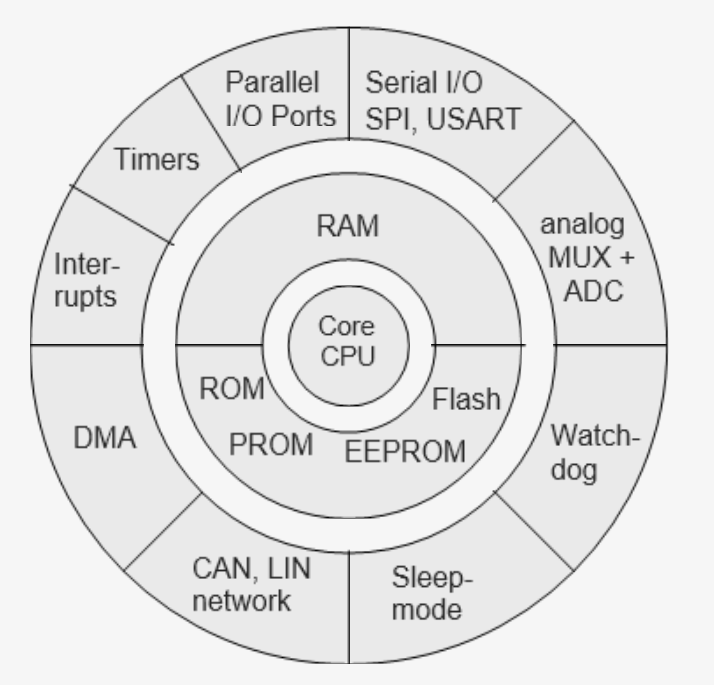
\includegraphics[width=8cm, height=7.5cm]{Images/image160.png}
    \caption{Layer model of a microcontroller (single chip) or a Microprocessor (more chips)}
    \label{fig:Fig 112}
    \end{figure}
\os{\newpage}

The microprocessor cores are often common CPU types used in the past as microprocessors. e.g. formerly: Motorola 680x0, 32 bit microprocessor (+ multi-board bodies)Today: Freescale "Coldfire" microcontroller = 68k CPU + integrated peripherals. \\

The single-chip solutions of modern microcontrollers are very cost effective and efficient, with already well-proven software $\rightarrow$ single chip solutions become more and more popular !\\

Microcontrollers are frequently used mobile, therefore energy management is of great importance (sleep mode).\\

With higher integration densities, microcontrollers are found today even with floating point or DSP - features (like integrated Multiply Accumulate hardware) for fast computation of digital filters.\\

Micro-controllers, as typically used in industrial applications have complex peripheral units like communication controllers for the CAN or LIN network.\\

The physical layer (ISO layer 1) of these networks though, is still implemented with external driver chips which, in high-voltage-technology (typ. 40V), while micro-controller chips are usually implemented in 5 V or 3.3 V technologies.\\

\textbf{Example}: AVR micro-controller AT90CAN

    \nsl{\begin{figure}[h]
    \centering
    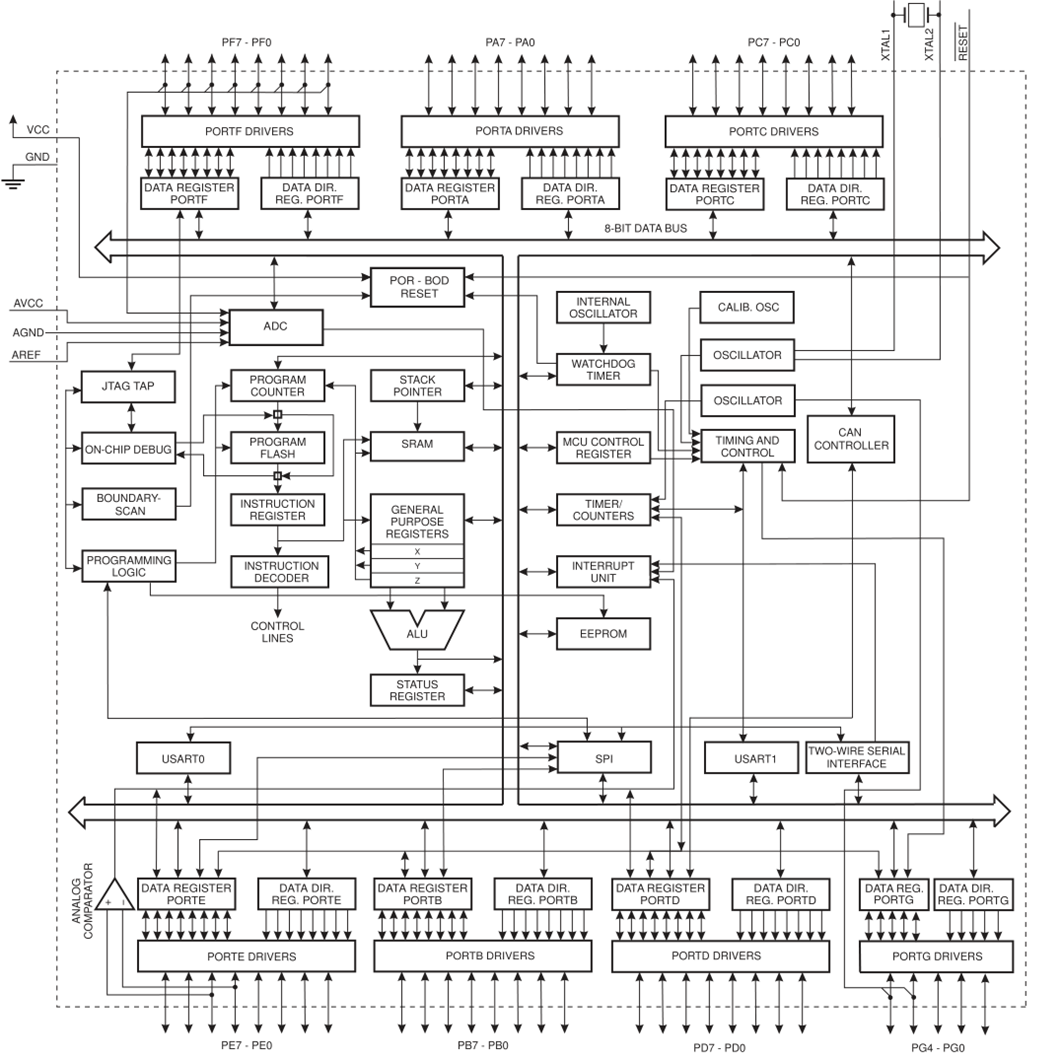
\includegraphics[width=15cm, height=16cm]{Images/image29.png}
    \caption{Layer model of a micro-controller (single chip) or a Microprocessor (more chips)}
    \label{fig:Fig 113}
    \end{figure}}
    
    \os{\begin{figure}[h]
    \centering
    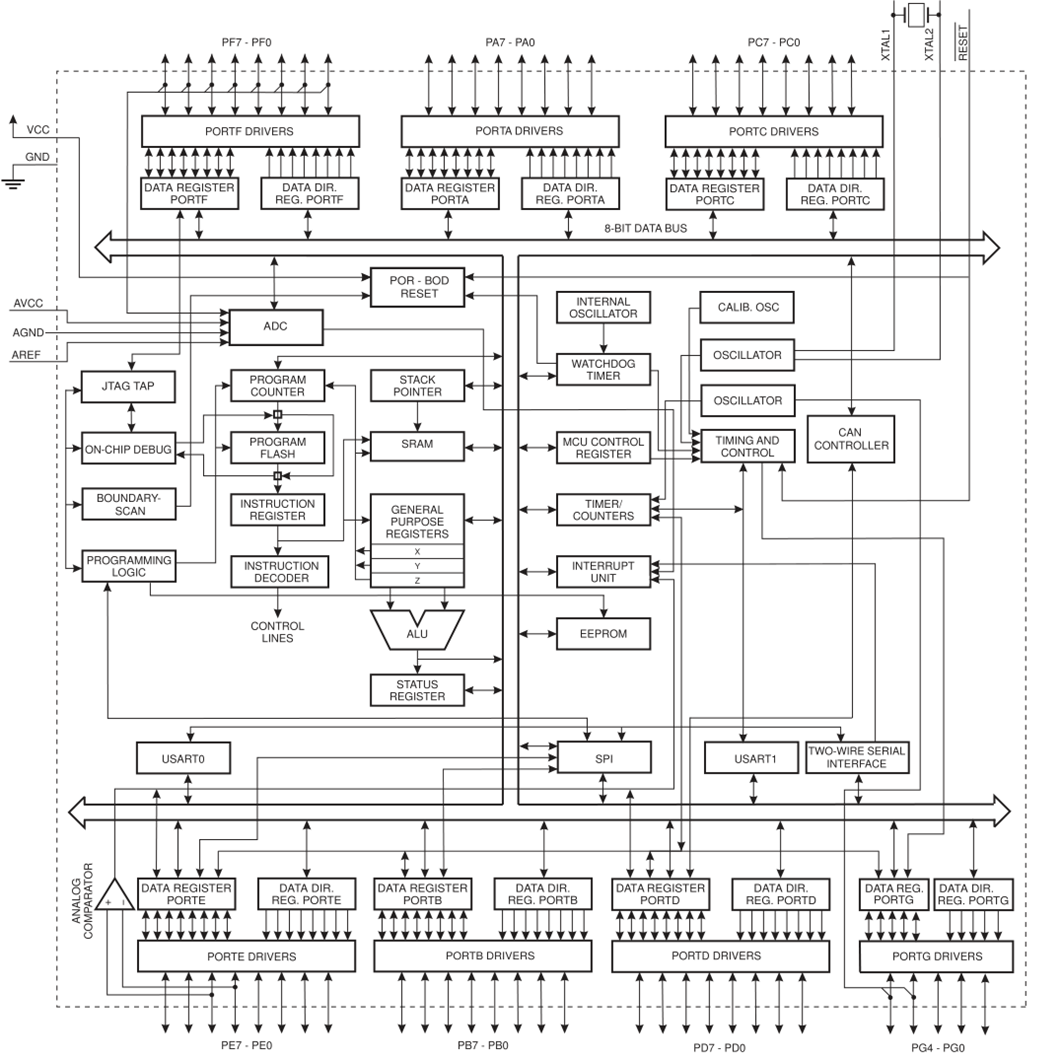
\includegraphics[width=14cm, height=10.2cm]{Images/image29.png}
    \caption{Layer model of a micro-controller (single chip) or a Microprocessor (more chips)}
    \label{fig:Fig 113}
    \end{figure}}
    
    \nsl{\begin{figure}[h]
    \centering
    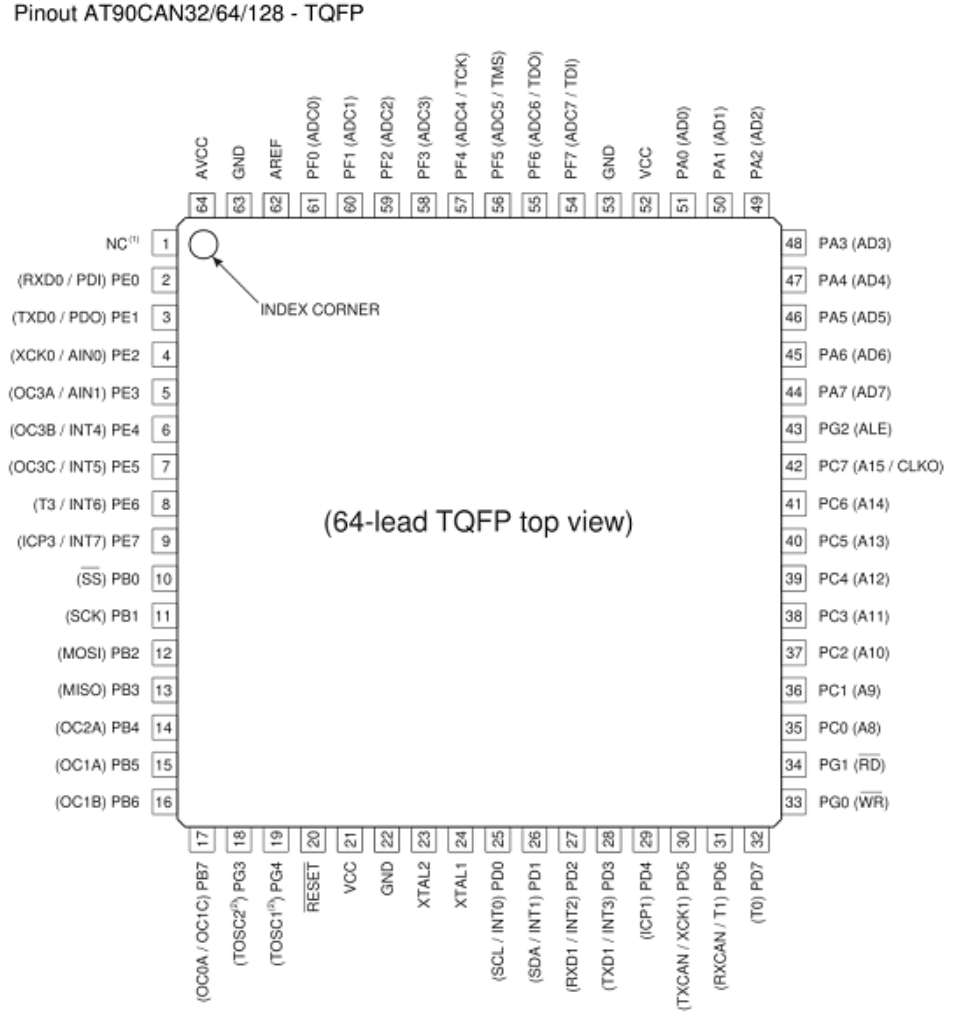
\includegraphics[width=5cm, height=5cm]{Images/image161.png}
    \caption{TQFP plastic housing 9 x 9 mm}
    \label{fig:Fig 114}
    \end{figure}}
    
    \os{\begin{figure}[h]
    \centering
    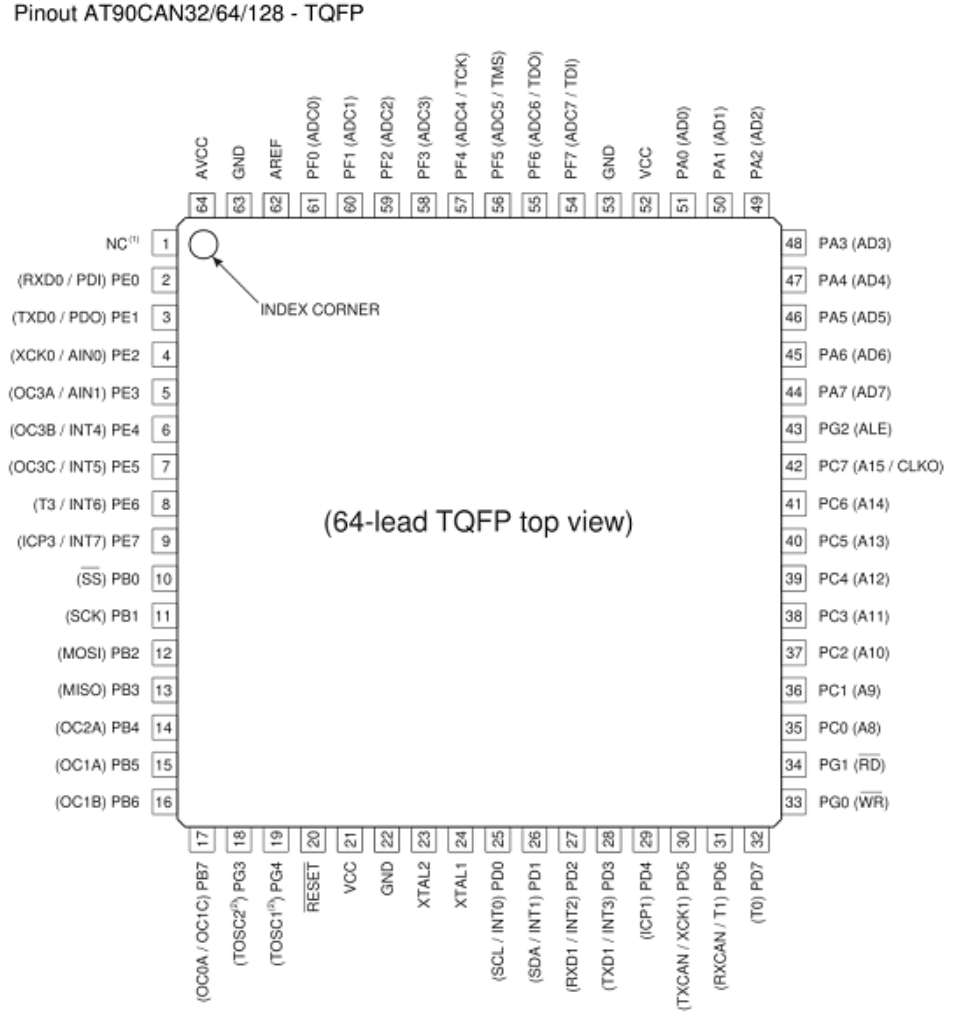
\includegraphics[width=10cm, height=10.2cm]{Images/image161.png}
    \caption{TQFP plastic housing 9 x 9 mm}
    \label{fig:Fig 114}
    \end{figure}}

\os{\newpage}
price $\mathrm{\approx}$ 1-2 $\texteuro$ (2009, in larger volumes).

\nsl{\newpage}

\section{Timers and Counters}

 \begin{figure}[h]
    \centering
    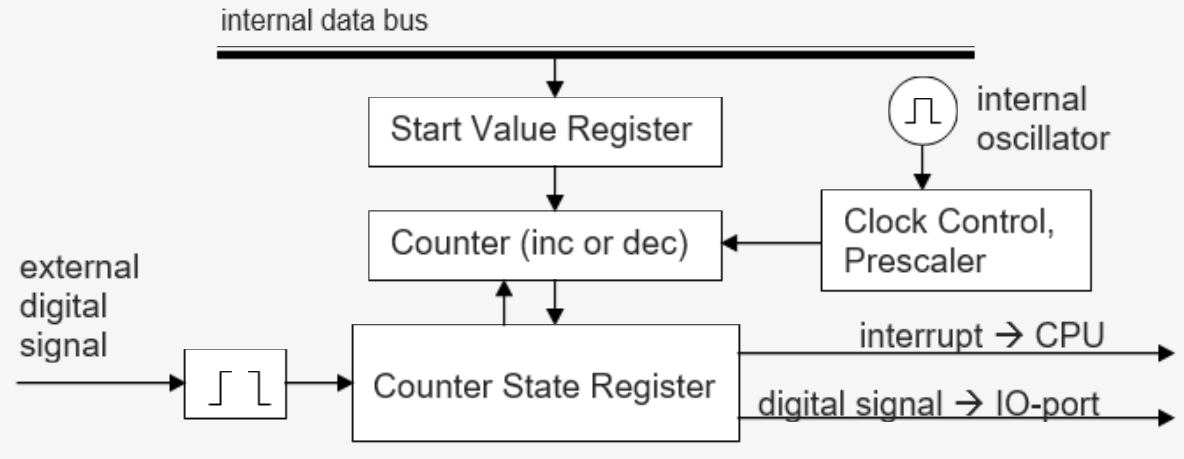
\includegraphics[width=14cm, height=5cm]{Images/image162.png}
    \caption{Basic structure of a timer-counter unit (CPU independent hardware)}
    \label{fig:Fig 115}
    \end{figure}

Timers and counters are very important components for real-time operation: Fed from an internal (RC) or external (quartz, ceramic resonator) oscillator, interrupts can be triggered with minimal delay, if

\begin{itemize}
\item  Internal events are true, like equality to a predetermined counter value.
\item  External events, like a rising or falling slope of a digital signal applied to some port can be stored as the count for this event in a register, and measuring at a later time as the time (counts) between such events.
\end{itemize}

Other important applications of the timer are PWM (Pulse Width Modulation) timers whose period length is usually fixed and the pulse width in terms of a short-term average can be controlled by a control register.\\

\nsl{The short-term average value is changed, and an analog signal can be measured after an analog low pass filter. This filtering effect can be done for example by the inductance (winding) an electric motor, which filters the square wave voltage to a DC to a short time average with the same short-term arithmetic mean.\\}
\newpage

\textbf{Example}: Periodic Event with AVR TCNT0 Hardware Timer  ISR(SIG\_OVERFLOW0) (similar to the "AVR Timer Interrupts" exercise in the RTP-Lab)\\

\begin{lstlisting}[style=mystyle, language=c]
#include	<avr\io.h>		  // AVR Register and constant definitions
...                       // (.. like #define TCNT0 0x32)
static unsigned int cnt;  // the timeslice counter
#define TCNT_PRELOAD 62   // for f_timeslice = 2 kHz 

void init() {
	...
	CLKPR = 8;              // prescaler Value
	TCCR0B |= (1 << CS01);  // Timer clock = system clock / CS
	                     	// CS = [1 8 256] mit [CS0 CS1 CS2]
	TCNT0 = TCNT_PRELOAD;   // Timer 0 Preload Value
	...
	cnt = 0;                // init timeslice counter
}

ISR(SIG_OVERFLOW0)        // this function is called at timer 0 overrun
{                         // f_timeslice = fosc/CS(prescale)/TCNT_PRELOAD
	TCNT0 = TCNT_PRELOAD;   // next cycle Timer Preload Value (normal mode)
	// time slice scheduling: 1/TTs = f_timeslice
	if (cnt & 1) {
	// the 2 time slice: 2*TTs (1 ms)
	fastTask();                   
  } else if ((cnt & 0x03) == 2) {
	// the 4 time slice: 4*TTs (2 ms)
	slowTask();          
  }
  cnt++;
}

int main(void)  // is executed after a reset
{
	init();        
	do {
	} while (1);		// endless mainloop
}

\end{lstlisting}

    \begin{figure}[h]
    \centering
    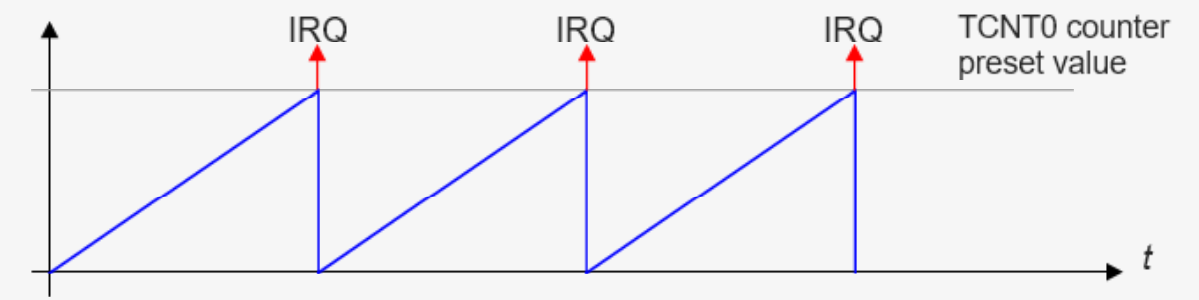
\includegraphics[width=12cm, height=3.5cm]{Images/image163.png}
    %\caption{}
    \label{fig:Fig 116}
    \end{figure}

\newpage
\section{Watchdog}

The term watchdog is used for a component of a system, which monitors the function of other components. If a possible malfunction is detected, this can be either 

\begin{itemize}
\item  a signal according to system specifications (e.g. air bag warning light), or, 
\item  appropriate steps are taken to fix the problem (e.g. reset).
\end{itemize}

Specifically watchdogs in microcontroller-controlled electronic devices are used to avoid a complete failure of the device through \textbf{\textit{software failure}}, or to take mitigating or workarounds. In most cases these are so-called time-out watchdogs, similar to a \textbf{\textit{dead-man's switch}} with a locomotive.\\

\os{\newpage}

{\rot\bf 1. Software-Watchdog}\\

The software watchdog is an examining task running on the microcontroller. The watchdog checks, if all important tasks are executed correctly within in a given time frame, or, if a task needs an inadmissible long process time. This functionality can be realized by setting timeouts for individual tasks to avoid locks, if supported by the RTOS.

{\rot\bf 2. Hardware-Watchdog}\\

Prevents the failure of an microcomputer system by triggering a special watchdog timer (hardware) by the software (one or more tasks) triggers at regular time intervals, to announce that the software still works properly (see AT90mega). With missing triggers, the watchdog timer resets the micro-controller ($\mu$C).

    \begin{figure}[h]
    \centering
    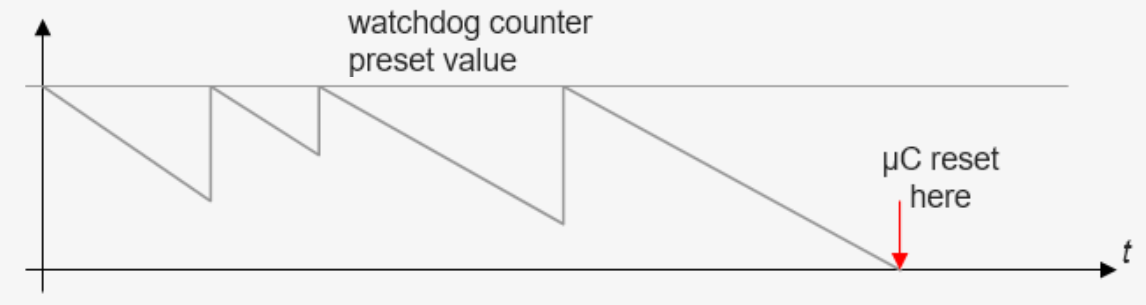
\includegraphics[width=12cm, height=4cm]{Images/image164.png}
    %\caption{}
    \label{fig:Fig 117}
    \end{figure}

To achieve even higher security against errors in the $\mu$C, the same functionality as the internal watchdog timer can be realized by an external watchdog module, which is independent of the $\mu$C supply and its clock. \\

The watchdog module is a hardware counter with a separate integrated clock generation. The counter is set at regular intervals by the software through an I/O port to a predetermined pre-set value.\\

The counter is decremented in watchdog module, if it ever reaches 0, it may have come to a deadlock or some other critical situation within the software, which was not debugged before (\textbf{software failure (?)}). \\

However, the watchdog will reset the $\mu$C device to its defined initial state (as with power-on), such that the software system can work properly again.\\

\os{\newpage}

{\rot\bf Intelligent Watchdog (with increased security requirements)}\\

With an intelligent watchdog, the micro-controller software has to answer a challenging message from an external watchdog correctly in an expected way  challenge-response approach\\

In case of failure not only a reset of the micro-controller is generated, but the watchdog usually brings the whole system into a safe condition -regardless of the apparently uncontrolled micro-controller.\\

\textbf{Example}: Intelligent watchdog for the electronic accelerator (e-gas) in the car:\\
By careful choice of the challenges caused by arithmetic operations, the CPU's internal modules (ALU, program memory, working memory and registers are monitored).

\section{DA Converters}

A  voltage DA converter (DAC) converts an integer number \textit{Z} (in a digital computer), into a voltage. The voltage \textit{U${}_{a}$} is proportional to the number \textit{Z} (with a linear DAC), by\\

\textit{U ${}_{a}$} = Z $\mathrm{\bullet}$ \textit{U ${}_{LSB}$}\\

\textit{U${}_{LSB}$} is the voltage for the least significant bit (LSB), thus the voltage according to \textit{$Z$} = 1.\\
\os{\newpage}
One can distinguish three fundamentally different methods:

\os{\hspace{2cm}}

    \nsl{\begin{figure}[h]
    \centering
    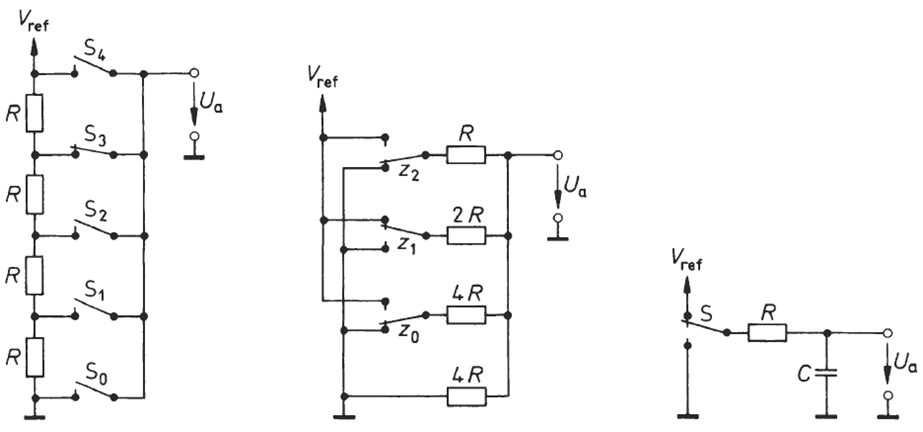
\includegraphics[width=14cm, height=6cm]{Images/image31.png}
    \label{fig:Fig 118}
    \end{figure}}
    
    \os{\begin{figure}[h]
    \centering
    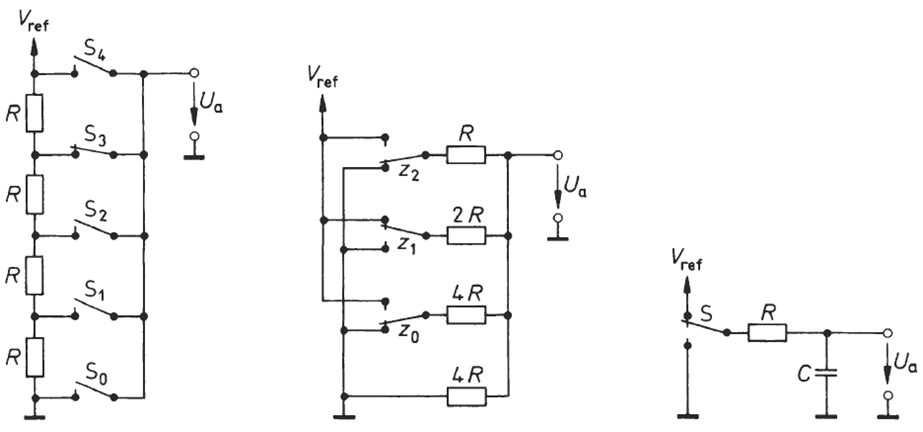
\includegraphics[width=15cm, height=8cm]{Images/image31.png}
    \label{fig:Fig 118}
    \end{figure}}

\os{\newpage}

\begin{enumerate}
\item \textbf{Parallel (direct) method} with a voltage divider all possible output voltages are provided. With a 1-of-n decoder then closes the right switch, the desired output voltage is associated with.

\item \textbf{Successive approximation method} (SAR)each bit is associated with a switch. Using appropriately weighted resistors (often R-2R) the output voltage is set-up by a loaded DC voltage divider.

\item \textbf{Counting methods} (PWM) requires only a single switch, which is periodically opened and closed. Its duty cycle is controlled by a pulse width modulator such, that the arithmetic mean of the output voltage corresponds to the desired value.\\

The comparison of the three methods shows that the parallel method (a) requires \textit{Z${}_{max}$} switches, the SAR type needs ld(\textit{Z${}_{max}$}) switches, and the PWM type only one switch. \\

\nsl{Because of the large number of switches required for high precision DACs, the parallel methods are used rarely. The counting methods become increasingly important, because here the pulse width modulator is an easy-to-integrate digital circuitry. If it operates at a frequency which is much higher than the sampling frequency (\textbf{oversampling}), only a simple \textbf{analog} low-pass filter is necessary.}
\end{enumerate}
\newpage

\subsection{Successive Approximation DAC}

    \begin{figure}[h]
    \centering
    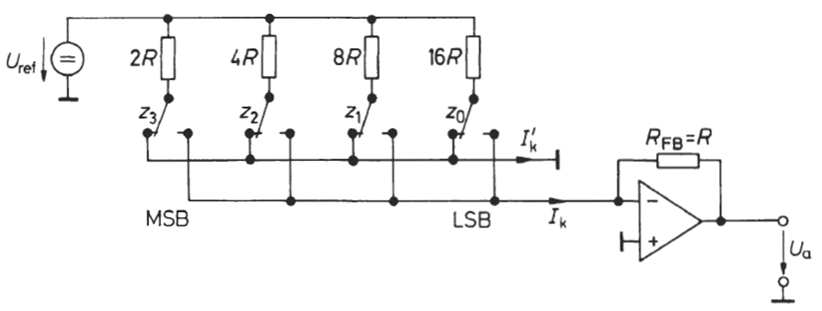
\includegraphics[width=14cm, height=7cm]{Images/image32.png}
    %\caption{}
    \label{fig:Fig 119}
    \end{figure}

here: \textit{Z}${}_{max}$ = 15\\

\os{\newpage}

{\rot\bf DAC with R-2R network} (can be realized in CMOS technology)

    \begin{figure}[h]
    \centering
    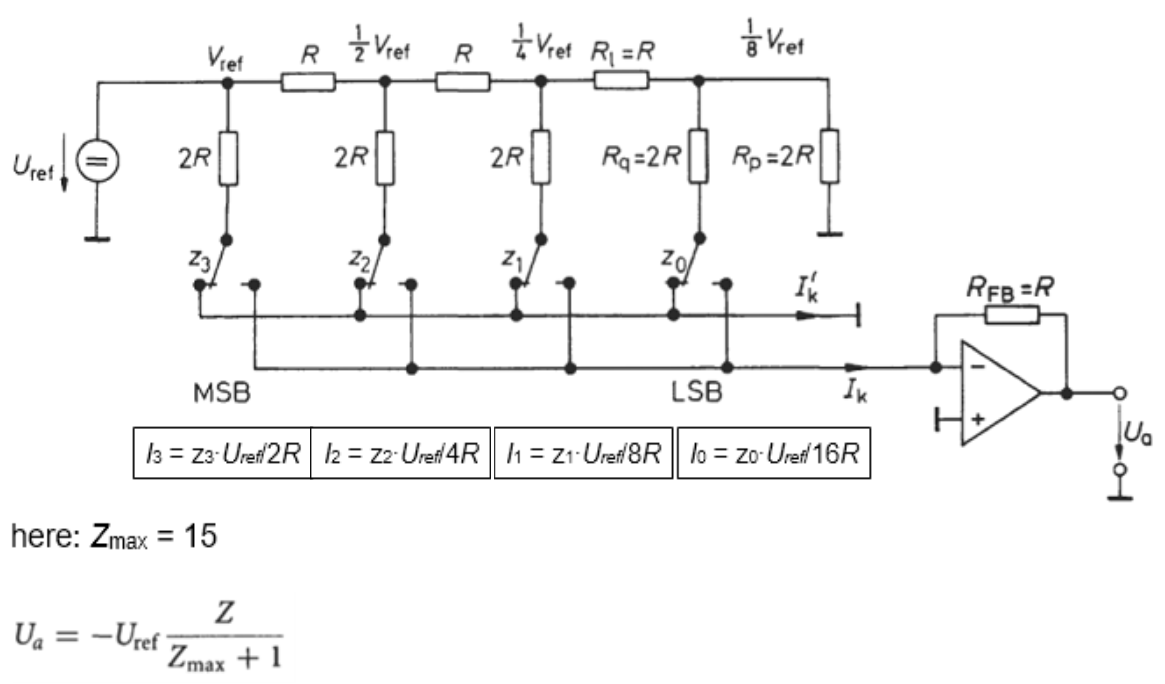
\includegraphics[width=14cm, height=7cm]{Images/image166.png}
    %\caption{}
    \label{fig:Fig 120}
    \end{figure}

Both SAR type DA converters shown above, are found in separate integrated circuits, often with a serial interface to a $\mu$C. \\

e.g. LTC1453 - Dual 12-Bit DACs in SO-8 package (SPI-Interface).\\

\nsl{SAR type DACs are rarely found integrated with a micro-controller chip (exception: NXP-LPC1766 with integrated 10-bit SAR DAC). Many applications are realized with PWM DACs.}
\newpage

\subsection{DA Converter (PWM)}

Pulse-width modulation (PWM) is a modulation, where a physical quantity (e.g. an electric voltage) switches between two values at a constant frequency \textit{f}  = \textit{T}${}^{-1}$, withthe duty cycle ratio \textit{d} = \textit{D} / \textit{T} of the modulated digital signal, with \textit{D} as width of a pulse.\\

\textbf{Example 1}:  PWM-DA converter with \textit{U ${}_{a}$}(\textit{t}) generated at a $\mu$C-Port with \textit{T} $\mathrm{<}$ $\mathrm{<}$ ,  = \textit{R} $\mathrm{\bullet}$\textit{C}.

    \begin{figure}[h]
    \centering
    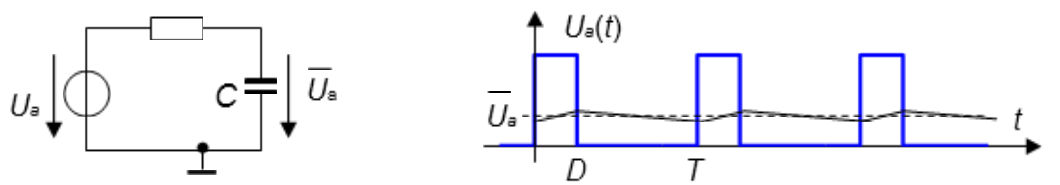
\includegraphics[width=12cm, height=3cm]{Images/image167.png}
    %\caption{}
    \label{fig:Fig 121}
    \end{figure}

\textbf{Example 2}:  PWM control of an R-L impedance with \textit{T} $\mathrm{<}$ $\mathrm{<}$ \textit{L}/\textit{R}.

    \begin{figure}[h]
    \centering
    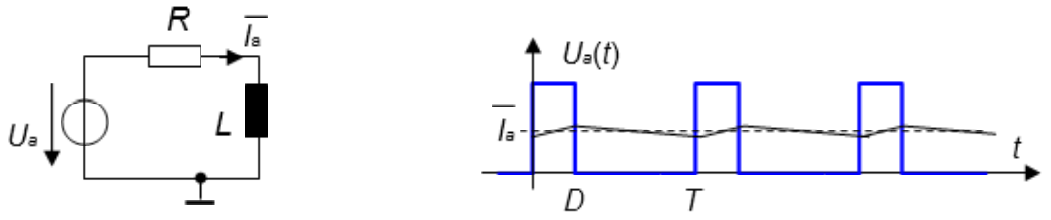
\includegraphics[width=12cm, height=3cm]{Images/image168.png}
    %\caption{}
    \label{fig:Fig 122}
    \end{figure}

\textbf{Example 3}:  PWM Control with Direction Control of a DC-Motor  Full Bridge.

    \begin{figure}[h]
    \centering
    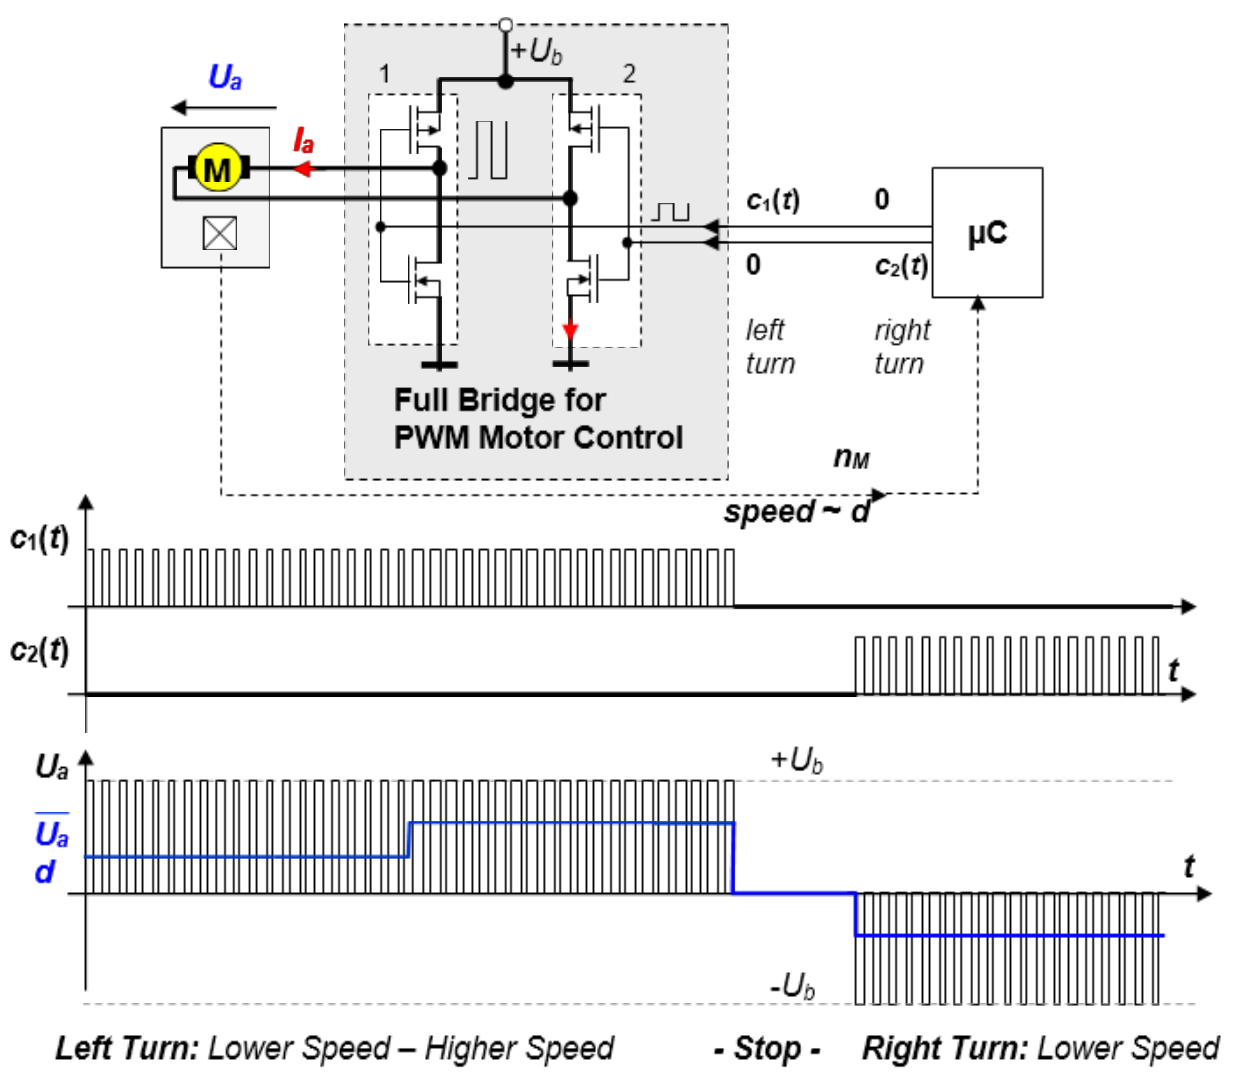
\includegraphics[width=15cm, height=10cm]{Images/image169.png}
    %\caption{}
    \label{fig:Fig 123}
    \end{figure}
\newpage

\textbf{ Example 4}:  PWM control with a time fiunction of the duty-cycle.

    \begin{figure}[h]
    \centering
    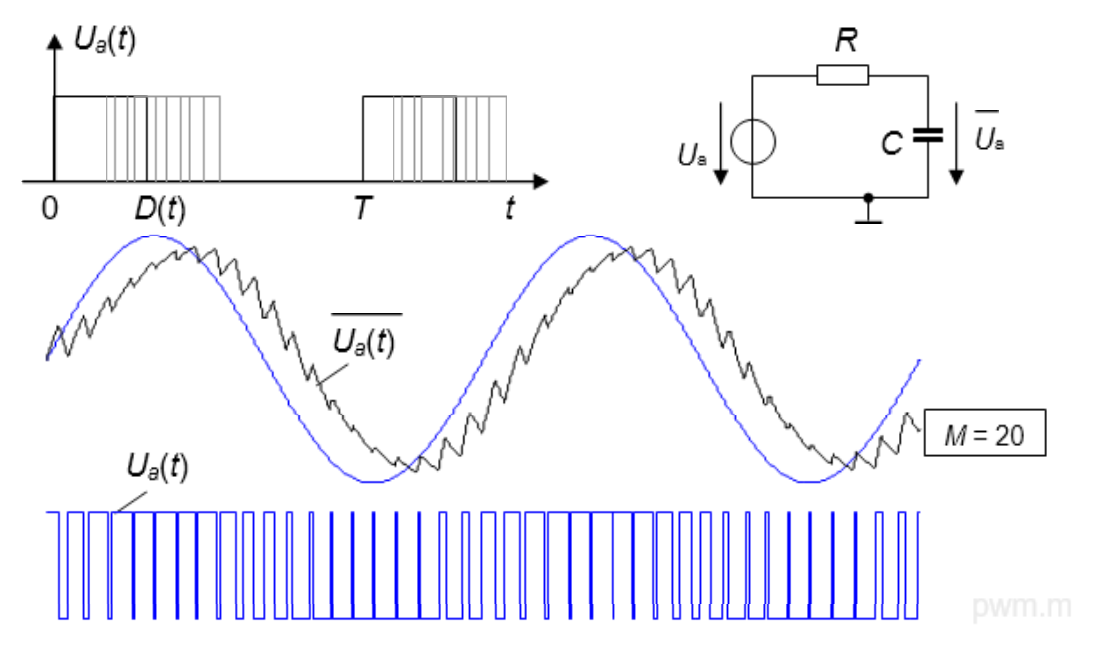
\includegraphics[width=14cm, height=7.5cm]{Images/image170.png}
    %\caption{}
    \label{fig:Fig 124}
    \end{figure}

A PWM signal is demodulated, generally, by a low pass filter. The resulting demodulated technical quantity \textit{d}(\textit{t}) is the short-term mean and thus, the mean height of the area under the modulated quantity \textit{U${}_{D}$}(\textit{t}). With an integration time constant  = \textit{R$\bullet$C} \\

 $U_{a} (t)\approx U_{D} (t)=\frac{1}{T} \int _{0}^{T}U_{D} (t)\, dt =\frac{D(t)}{T} \cdot \hat{u}=d(t)\cdot \hat{u}$  (4.1) \\

the RC lowpass acts as an integrator, if \textit{T} $\mathrm{<}$ $\mathrm{<}$ , or the PWM frequency is high compared to the bandwidth and the maximum frequency of the analog signal (oversampling ratio \textit{M}). \\

$\rightarrow$ The higher the time-constant related to the PWM periodic time, the smaller the "ripple"-amplitude.\\

In power electronics PWM is widely used, because the power dissipated into heat in the switch (\textit{P${}_{S}$ = U${}_{S}$}·\textit{I${}_{S}$}) can be minimized close to 0, if the switch is either \textbf{fully closed} (\textit{U${}_{S}$} = 0, \textit{I${}_{S}$} $\mathrm{\neq}$ 0) or \textbf{fully open} (\textit{U${}_{S}$} $\mathrm{\neq}$ 0, \textit{I${}_{S}$}  = 0).

    \begin{figure}[h]
    \centering
    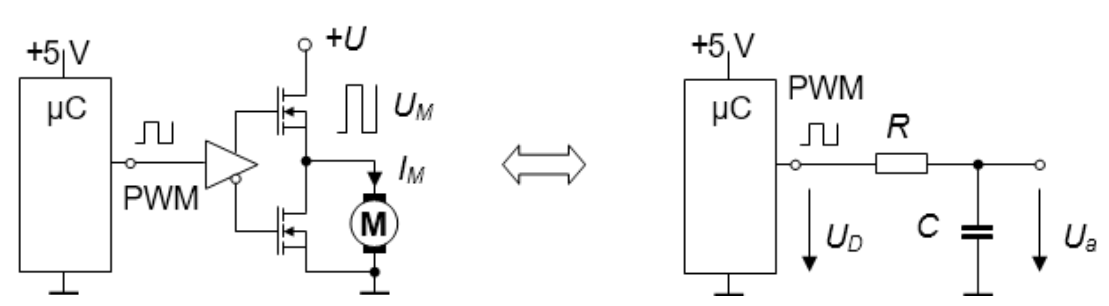
\includegraphics[width=14cm, height=4cm]{Images/image171.png}
    %\caption{}
    \label{fig:Fig 125}
    \end{figure}
    
\os{\newpage}

A vivid example of PWM modulation is a pair of switches (realized as power MOSFETs), which is used to control the DC motor of a drive by constantly switching on and off.\\

The higher the duty cycle ratio \textit{d} = on-time / (off-time + on-time) of the switch, the higher the average speed. Due to lowpass characteristics of the motor, the motor acts as a low-pass filter with time-constant  = \textit{L ${}_{a}$}/\textit{R ${}_{a}$} $\mathrm{\sim}$ 20 ms. Thus, speed cannot follow a 20 kHz PWM frequency (as a typical PWM frequency at 20 kHz (audio limit) is used,  \textit{T} = 50 $\mu$s). Since \textit{T} $\mathrm{<}$ $\mathrm{<}$, the motor speed is proportional to the average duty cycle \textit{d}. \\

Power loss with specified \textit{R${}_{on}$} of a half-bridge:     \textit{P${}_{s}$ }= \textit{I${}_{M}$}${}^{2}$ \textit{R${}_{on}$}Example: \textit{R${}_{on}$} = 5 , \textit{I${}_{M}$} = 10 A  \textit{P${}_{s}$} = 0.5 W    (very low power loss)\\

\textbf{Example} (from examination WS2010):\\

In a real-time program for a microcontroller a PWM DAC shall be realized for generating 2 different analog voltages \textit{U${}_{a}$}${}_{1}$ and \textit{U${}_{a}$}${}_{2}$ by means of a programmable PWM timer with period \textit{T} = 50 $\mu$s (20 kHz), and a 5 V digital output pin of the micro-controller, and an analog RC low-pass.

    \begin{figure}[h]
    \centering
    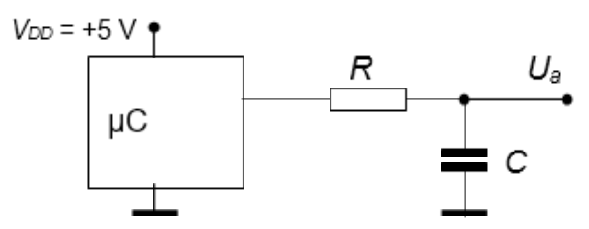
\includegraphics[width=7cm, height=3cm]{Images/image172.png}
    %\caption{}
    \label{fig:Fig 126}
    \end{figure}

Which pulse width \textit{D}${}_{1}$ (or \textit{D}${}_{2}$) must be programmed to get \textit{U${}_{a}$}${}_{1\ }$= 1 V (to get \textit{U${}_{a}$}${}_{2\ }$= 3 V) at the output of the RC-lowpass ?\\

with (4.1):  \textit{$\frac{D}{T} =\frac{U_{a} }{V_{DD} } $}  \\

\textit{D}${}_{1}$ = 1V /5V · 50 $\mu$s = 10 $\mu$s.  \\
\textit{D}${}_{2}$ = 3V / 5V · 50 $\mu$s = 30 $\mu$s.  \\  

What RC-time constant \textit{${}_{RC}$} is useful, if the voltage \textit{U${}_{a}$} is switched periodically between \textit{U${}_{a}$}${}_{1}$ und \textit{U${}_{a}$}${}_{2\ }$at a periodic time \textit{T${}_{on,off}$}  = 10 ms ? \\ 

$T_{on,off}=5$ $\tau$ $RC$ \hspace{1cm} $\rightarrow$ $\tau$ $RC=$  $T_{on,off}/5=2ms$ \\
$\tau$ $RC=$ $R.C >>T$ \hspace{0.80cm} $\rightarrow$ $2ms >> 50 us$ OK\\

$\rightarrow$ The lower the time constant, the higher the \textbf{PWM-ripple amplitude} ! \\

When switching the pulse durations \textit{D}${}_{1}$ (\textit{D}${}_{2}$) each 5 ms, one gets the signal \textit{U${}_{a}$}(\textit{t})

    \begin{figure}[h]
    \centering
    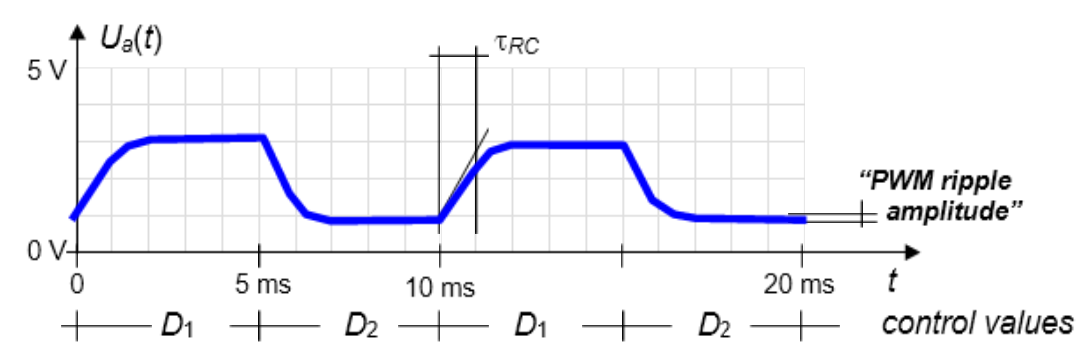
\includegraphics[width=10cm, height=4cm]{Images/image173.png}
    %\caption{DA Converter (Delta-Sigma Method)}
    \label{fig:Fig 127}
    \end{figure}

\subsection{DA Converter (Delta-Sigma Method)}

see 4.5.4

\section{AD Converters}

If an analog voltage shall be processed by a digital computer, that voltage must be translated into a corresponding number. This is the task is an analog-digital converter (ADC). With \textit{$Z$} as an integer number, proportional to the analog input voltage \textit{U}${}_{e}$\\

Z\textit{ }= \textit{U${}_{e}$} / \textit{U}${}_{LSB}$\\

this is called a linear ADC, this type is most widespread type (for more specific applications, there are also logarithmic ADCs).\\

\textit{U${}_{LSB}$} is the voltage unit for the least significant bit (LSB), that is the voltage corresponding to $\mathrm{Z}$ = 1, it is derived from an \textbf{\textit{accurate reference voltage}} \textit{U${}_{ref}$}.\\

One can basically distinguish four different methods:

\begin{enumerate}
\item  Flash-method (parallel method),  "word at a time"
\item  Successive-Approximation-method (SAR) "digit at a time"
\item  Counting methods "level at a time"
\item  Sigma-Delta methods
\end{enumerate}

There is a compromise between flash- and SAR-concerters: \textbf{cascade converters} ("half-flash converters"), which are not presented here. These converters provide high resolution at high sampling frequencies [Tietze]. Cascade converters behave like flash ADCs from the perspective of software.\\
\newpage

    \begin{figure}[h]
    \centering
    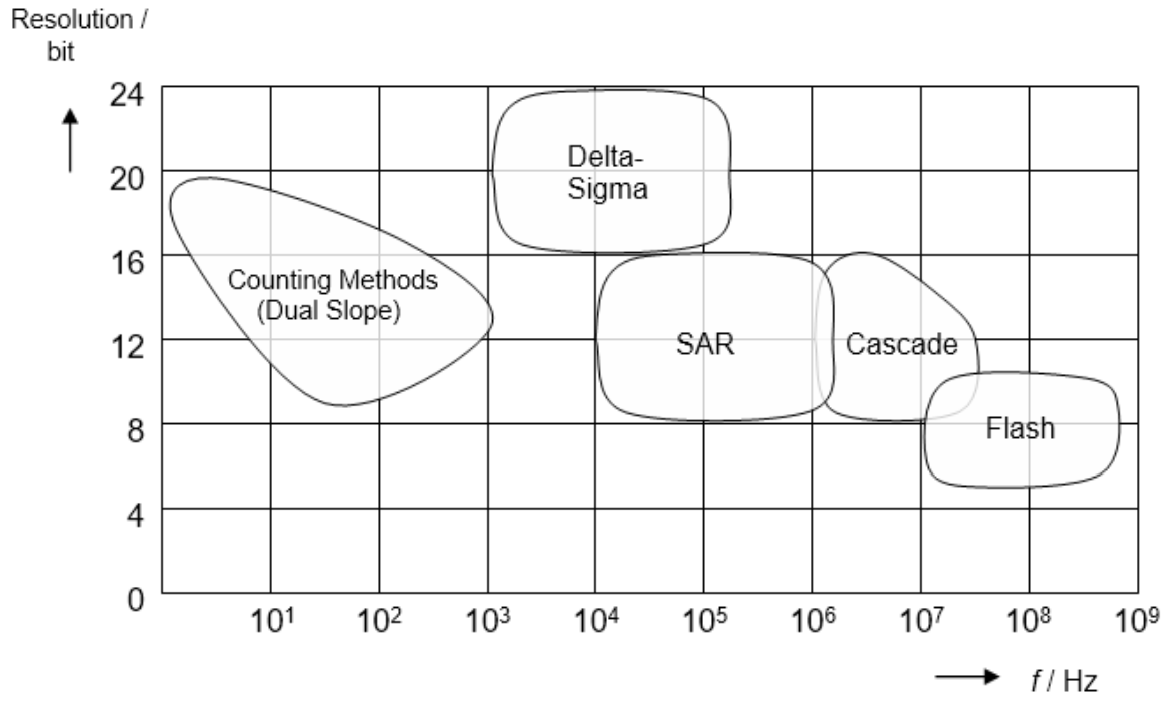
\includegraphics[width=11cm, height=6cm]{Images/image174.png}
    \caption{AD-Converters - Resolution and max. Sampling Frequencies}
    \label{fig:Fig 128}
    \end{figure}
    
\subsection{Flash-Method (parallel method)}

A flash ADC compares the input voltage simultaneously (in parallel) with \textit{n} reference voltages and states, and compares the interval between the unknown input voltage is beween. By this, one gets the full conversion in one step ("one word at a time"), very quickly.\\

However, the cost is very high, as is required for any possible number 1 .. \textit{Z${}_{max}$} a separate comparator is needed  for a measuring range 0-255 steps (8-bit), 255 comparators.\\

\textbf{Applications for flash ADCs:} Video conversion, Oscilloscope, radar, ...\\

\os{\newpage}

\textbf{Advantages}: 

\begin{itemize}
\item  very fast (conversion times of $\mathrm{\sim}$ 1 ns (8 bit, 600 MHz: TDA8718),or $\mathrm{\sim}$ 10 ns (10 bit, 75 MHz: AD 9060)
\item  due to the short aperture times, no sample \& holds circuits necessary the ADC result is obtained with a simple read from a data register: \textbf{z = get(ADC)}
\end{itemize}

\textbf{Disadvantages}:

\begin{itemize}
\item  no high resolutions available
\item  rel. expensive 
\item  analog semiconductor process  poorly implemented in CMOS technology
\end{itemize}
\os{\newpage}
    \nsl{\begin{figure}[h]
    \centering
    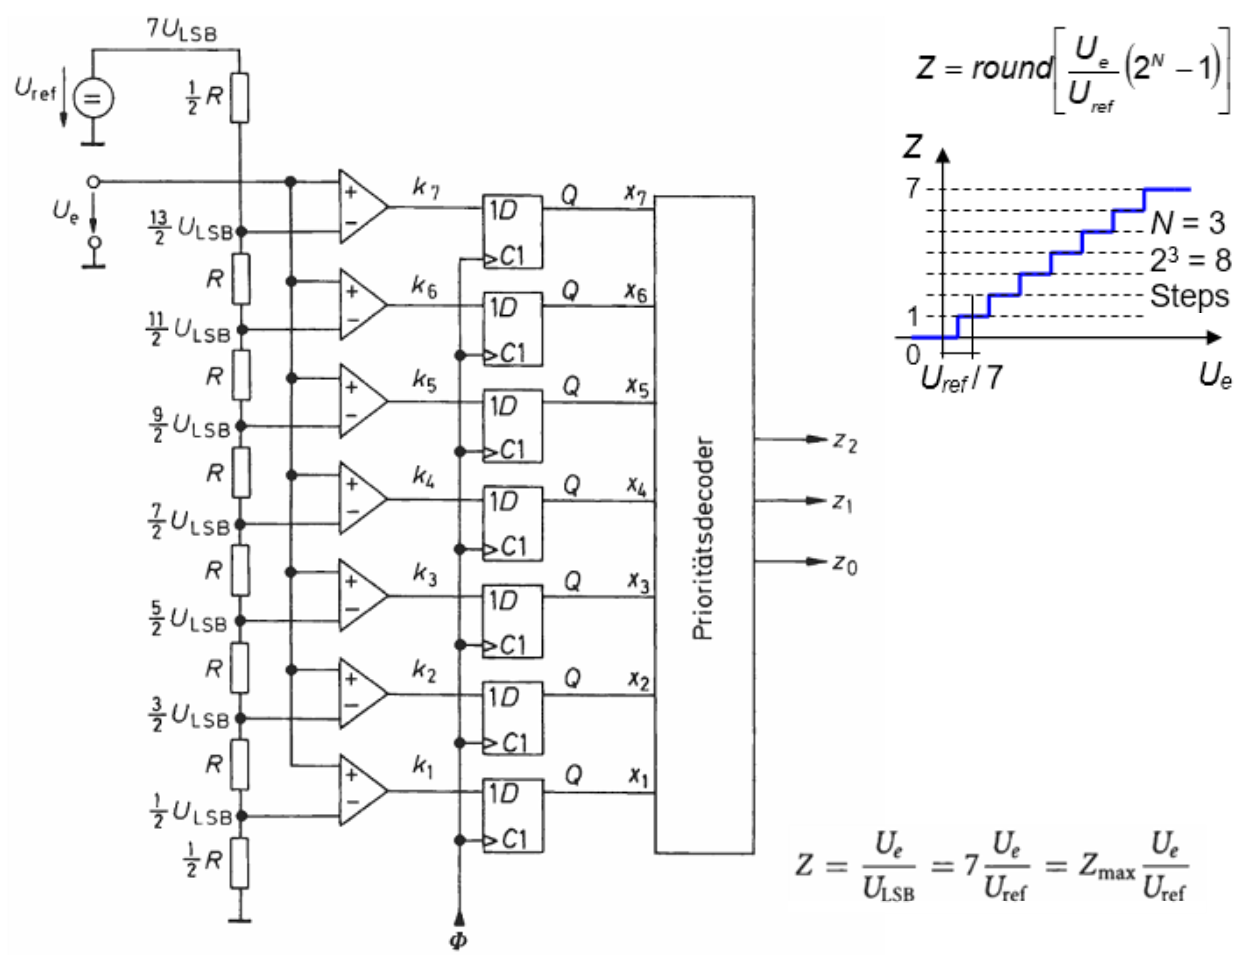
\includegraphics[width=15cm, height=9cm]{Images/image175.png}
    \caption{3-Bit Flash AD Converter (Parallel Method)}
    \label{fig:Fig 129}
    \end{figure}}
    
    \os{\begin{figure}[h]
    \centering
    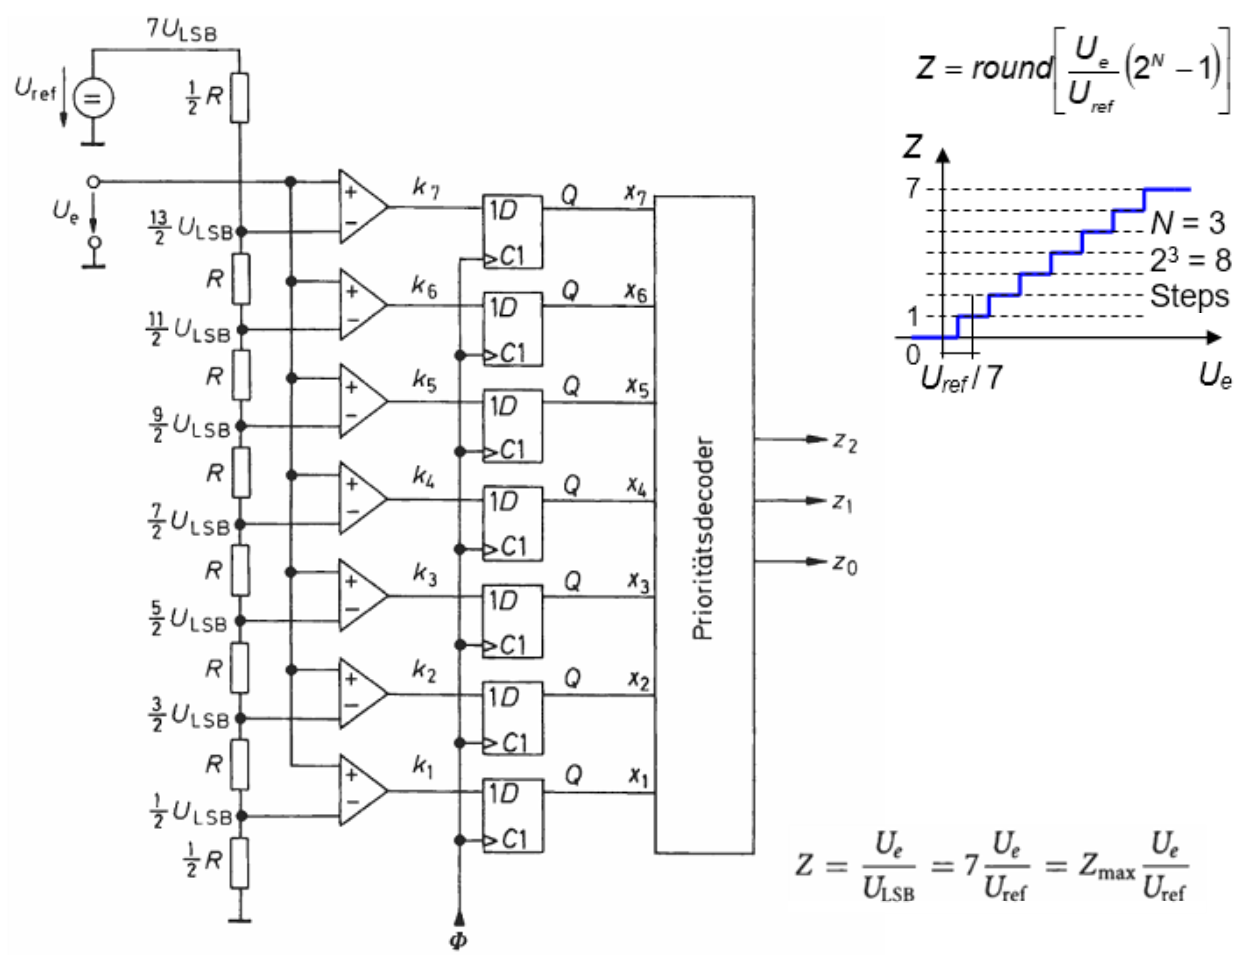
\includegraphics[width=15cm, height=10cm]{Images/image175.png}
    \caption{3-Bit Flash AD Converter (Parallel Method)}
    \label{fig:Fig 129}
    \end{figure}}

\os{\newpage}

\subsection{Successive Approximation Method}

With the successive approximation register (SAR) method, the final result is not produced in one step, but rather a sequence of results of successive comparison steps, similar to weighing a mass using a balance.Each digit, having a different significance, of the binary representation of the corresponding binary number is determined separately and successively.\\

It starts with the highest bit and determines whether the input voltage is higher or lower than the reference voltage for the highest bit. If it is greater, the voltage for the highest bit is subtracted. The rest is compared with the next bit, {\dots}. So as many comparison steps are needed, as bits are necessary to represent the number.

\[Z=round\left[\frac{U_{e} }{U_{ref} } \left(2^{N} -1\right)\right]\] 
    \begin{figure}[h]
    \centering
    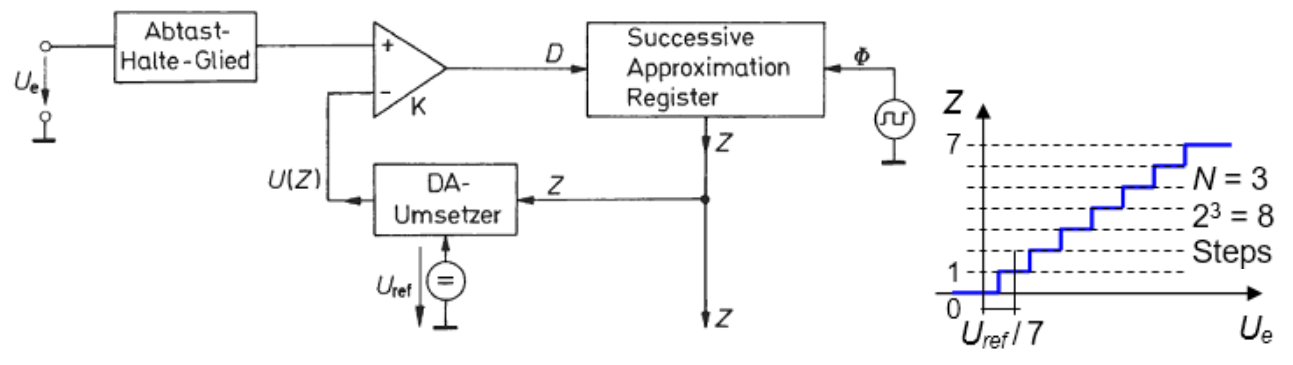
\includegraphics[width=13cm, height=4cm]{Images/image176.png}
    %\caption{}
    \label{fig:Fig 130}
    \end{figure}

\os{\newpage}

SAR-Converter with \textit{Z${}_{max}$} = 7 $\rightarrow$  3 steps. The SA-register is a digital sequential logic, which generates a voltage by a DAC a comparison voltage \textit{U}(\textit{Z}), and by the following sequential algorithm:

    \begin{figure}[h]
    \centering
    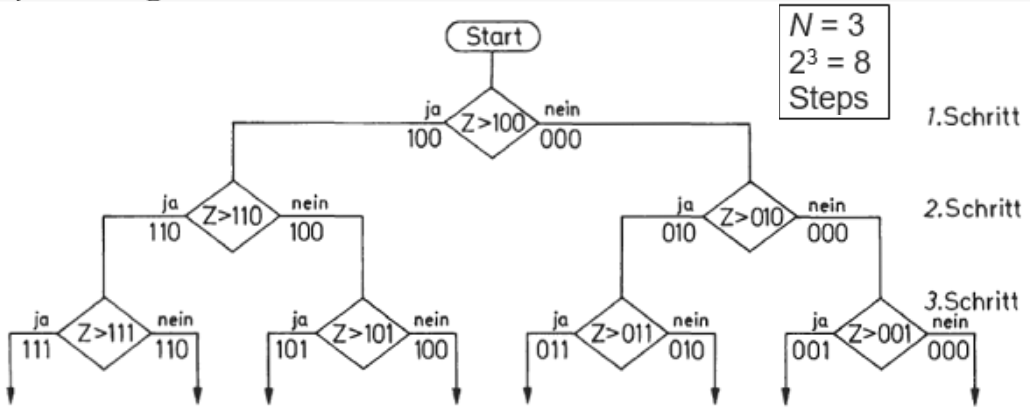
\includegraphics[width=12cm, height=4.5cm]{Images/image177.png}
    %\caption{}
    \label{fig:Fig 131}
    \end{figure}

\os{\newpage}

\textbf{Application}: Microcontroller, fast metrology, radar, ...\\

\textbf{Advantages: }

\begin{itemize}
\item fast and precise (conversion times $\mathrm{\sim}$ 1 $\mu$s (12 bit: TLV 5619)
\item  basically 1 comparator and digital circuitry necessary  \\
$\rightarrow$ realizable in CMOS, at reasonable cost, can be shrieked often integrated in micro-controllers
\end{itemize}

\textbf{Disadvantages: }

\begin{itemize}
\item \textbf{ }due to the rel. long conversion times, sample \& hold circuits are needed \\
$\rightarrow$ the SAR-ADC must be started first, activating the S\&H:     start\_ADC()  \\
$\rightarrow$ then, the ADC result is obtained with a read from a data register:   \textbf{z = get(ADC)}
\end{itemize}

\os{\newpage}

\textbf{Example: ADC readout with AVR micro-controller}\\

\begin{lstlisting}[style=mystyle, language=c]
unsigned char tmp_lo, tmp_hi;

ADCSRA |= (1<<ADSC);            // start AD-conversion ...
while ( ADCSRA & (1<<ADSC) ) {  // wait for AD to get finished
};
tmp_lo = ADCL;  							 // read AD-data register
tmp_hi = ADCH;

\end{lstlisting}

\subsection{Counting Method}

The simplest ADC method is the counting method. It is determined, how often some  reference voltage has to be added, until the input voltage is reached. The number of steps is equal to the result. If the largest representable number is \textit{n}, up to \textit{n} steps are needed to get the result.

    \begin{figure}[h]
    \centering
    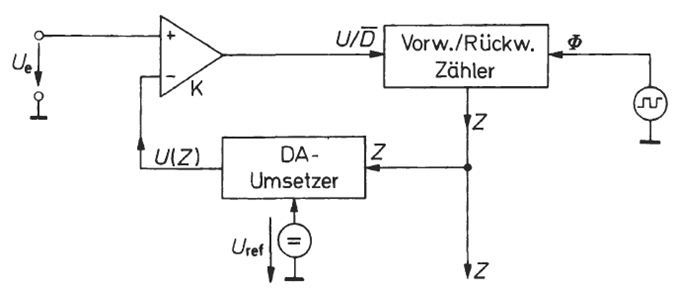
\includegraphics[width=10cm, height=4.5cm]{Images/image39.png}
    %\caption{}
    \label{fig:Fig 132}
    \end{figure}

AD conversion by the counting method requires low electronic circuit complexity, but conversion time is significantly larger as with other methods. It is usually between 1 ms and 1 s. This is sufficient for slowly changing signals, such as in temperature measurement or for laboratory instruments, which are read by eye (digital voltmeter). \\

The "Dual-Slope"-counting method has the greatest importance, for which the best accuracy can be achieved with little effort.\\

\textbf{Application}: Lab Measurement Devices\\

\textbf{Advantages:  }

\begin{itemize}
\item very precise (conversion times 1~ms ... 1~s \\
(HP, Keithley, Fluke -- Lab devices: 5.5 decimal digits and more)
\end{itemize}

\textbf{Disadvantages:  }

\begin{itemize}
\item due to the long conversion times, sample \& hold circuits are needed
\end{itemize}

\nsl{\textbf{Example}: Python Script for reading a measured voltage by GPIB:

\begin{tcolorbox}[colback=blue!5!white,colframe=blue!75!black]
see http://pyvisa.sourceforge.net\\
import visa\\
keithley = visa.instrument("GPIB::12")\\
print keithley.ask("*IDN?") 
\end{tcolorbox}

    \begin{figure}[h]
    \centering
    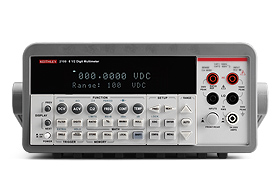
\includegraphics[width=5cm, height=3cm]{Images/image40.png}
    %\caption{}
    \label{fig:Fig 133}
    \end{figure}}
\newpage

\subsection{AD Converter (Delta-Sigma Method)}

A delta-sigma-ADC consists of a delta-sigma modulator which produces the so-called \textbf{\textit{bitstream}}, and a low pass filter in series.

\os{\hspace{1.5cm}
    \begin{figure}[h]
    \centering
    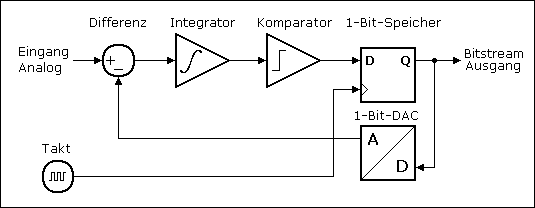
\includegraphics[width=14cm, height=6cm]{Images/image41.png}
    \caption{Delta-Sigma Modulator}
    \label{fig:Fig 134}
    \end{figure}}
    
    \nsl{\begin{figure}[h]
    \centering
    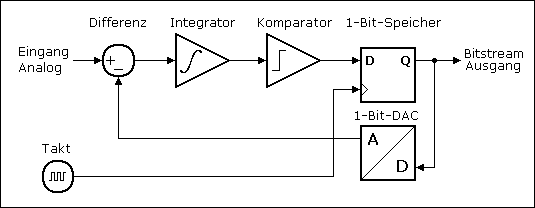
\includegraphics[width=12cm, height=4.5cm]{Images/image41.png}
    \caption{Delta-Sigma Modulator}
    \label{fig:Fig 134}
    \end{figure}}

    \begin{figure}[h]
    \centering
    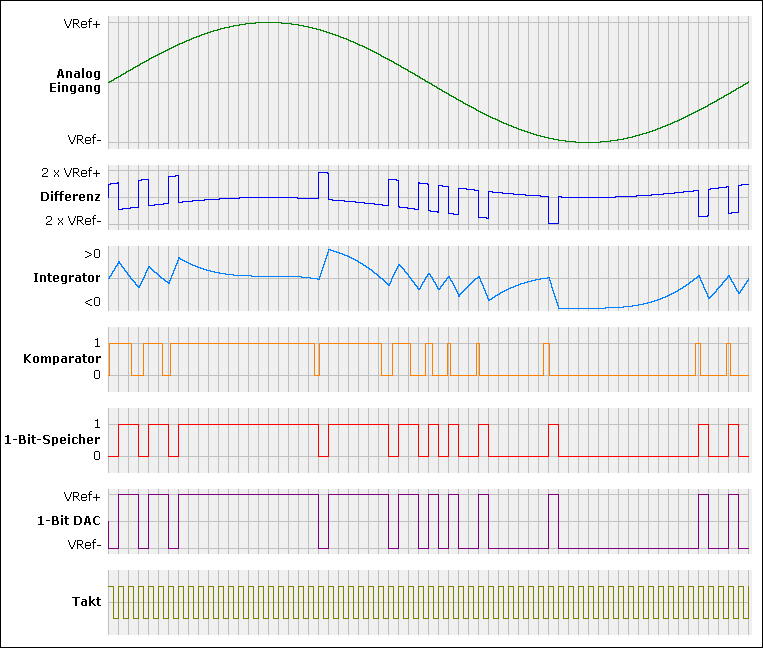
\includegraphics[width=15cm, height=10cm]{Images/image42.png}
    \caption{Signals with the Delta-Sigma Modulator}
    \label{fig:Fig 135}
    \end{figure}
    \os{\newpage} 
\nsl{The output signal at the 1-bit memory contains the analog signal with a resolution of only one bit, but with considerably higher frequency components (in the picture factor 64). This is referred as oversampling \textit{M} (here \textit{M} = 64). Since the original analog signal is included in the 1-bit signal as a short-term average, it can be obtained by a low pass filter as a very good approximation to the analog signal (see also section 4.4.2 PWM DACs):}
\nsl{\newpage}

\os{\newpage}
{\rot\bf Delta Sigma ADC}:

    \begin{figure}[h]
    \centering
    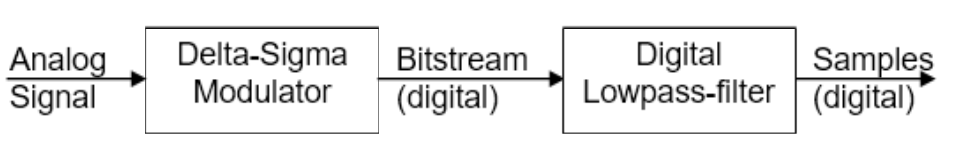
\includegraphics[width=10cm, height=1.5cm]{Images/image178.png}
    %\caption{}
    \label{fig:Fig 136}
    \end{figure}
    
Thus, the digital low pass filter realizes the short-term average (interpolation) on the 1-bit square wave signal with a high oversampling factor \textit{M}. Since both the input and the output of the filter are discrete-in-time and disctrete-in-value, this low-pass filter is realized as a digital filter (in hardware, an easy task with standard CMOS semiconductor technology).

    \begin{figure}[h]
    \centering
    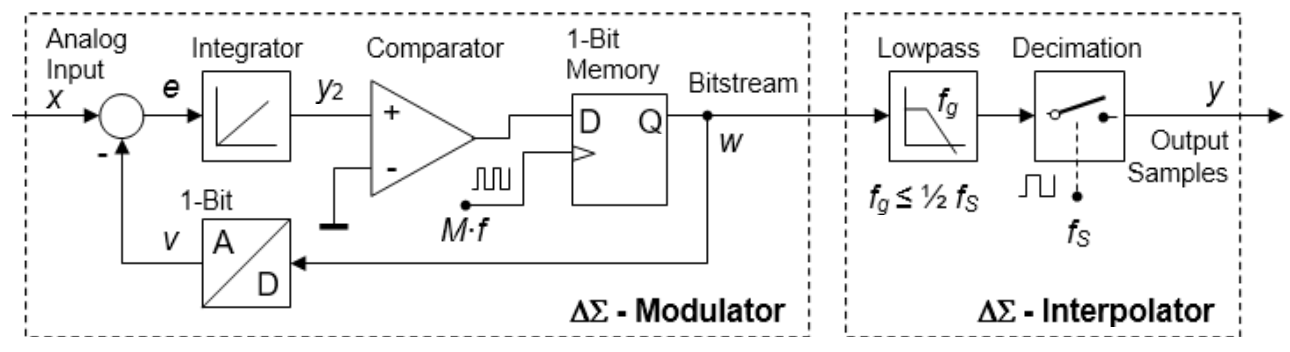
\includegraphics[width=15cm, height=4cm]{Images/image179.png}
    %\caption{}
    \label{fig:Fig 137}
    \end{figure}
    
    \begin{figure}[h]
    \centering
    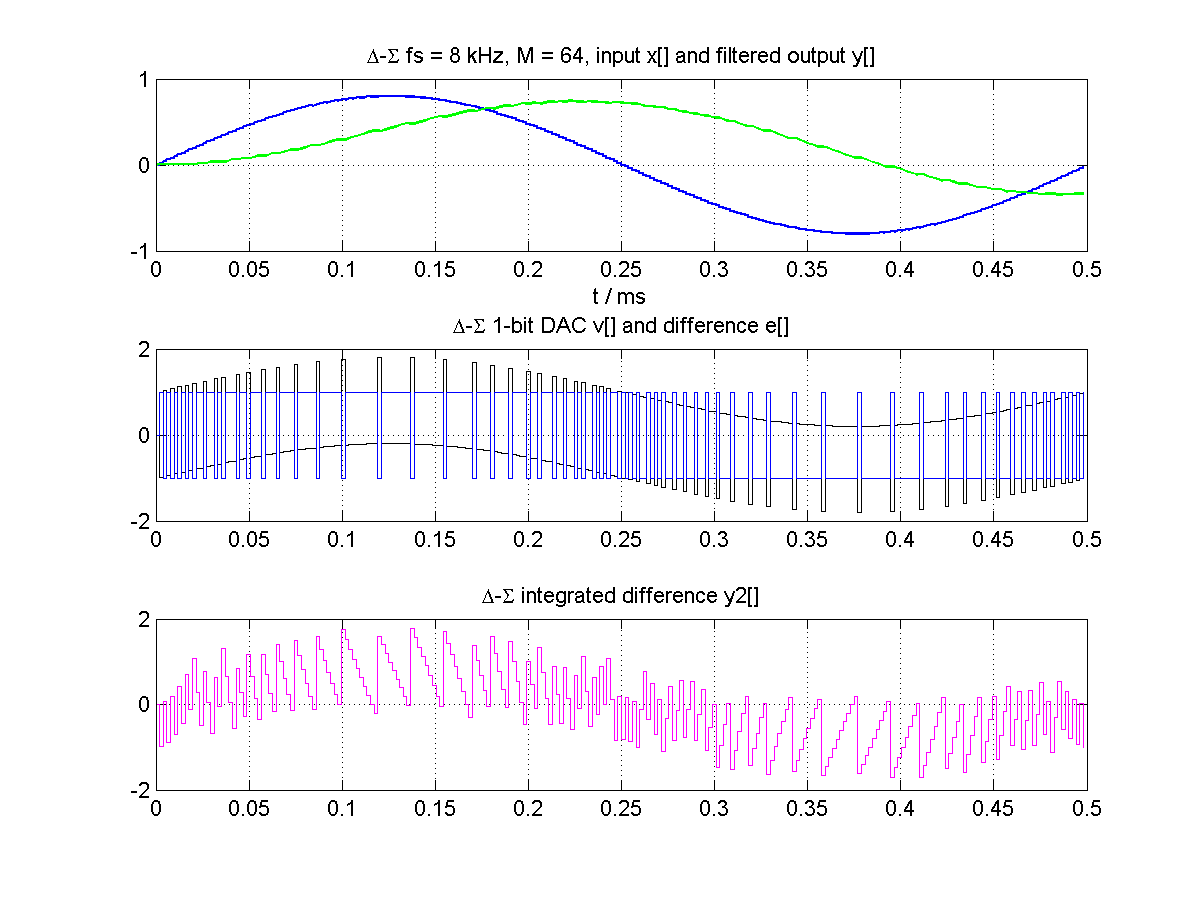
\includegraphics[width=15cm, height=10cm]{Images/image43.png}
    %\caption{}
    \label{fig:Fig 138}
    \end{figure}

Waveforms in a ADC with 8 kHz sampling frequency and 64-times oversampling. The low-pass filter is realized as a digital filter (usually as a FIR filter of high order). \\

A change of input- and output signal with the flowchart of the -ADC leads to a \\

{\rot\bf Delta-Sigma DAC}:\\

    \begin{figure}[h]
    \centering
    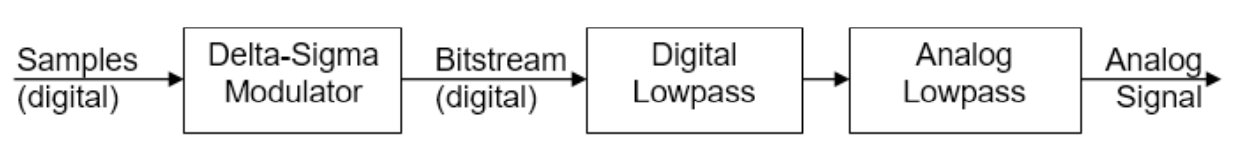
\includegraphics[width=14cm, height=2cm]{Images/image180.png}
    %\caption{}
    \label{fig:Fig 139}
    \end{figure}

The realization of the delta-sigma modulator is purely digital, the low pass filter is usually a combination of a high order FIR digital filter and a (quite simple) analog lowpass filter. With a -DAC no decimator is needed.\\

\textbf{Example}: For audio Delta-Sigma converters (ADC and DAC) resolutions of 16 to 24 bit at  sampling rates of 48 kHz are typical. The samples are processed in blocks of samples (typically 64-2048 values) using DMA ( section  4.6) for memory transfer.\\

\textbf{Advantages } of Delta-Sigma Converters:

\begin{itemize}
\item  fast, accurate AD- and DA- conversion possible
\item  no sample and hold circuits needed
\item  in addition to a single comparator only digital components
\item needed $\rightarrow$ can be highly integrated in CMOS technology
\end{itemize}

\textbf{Disadvantages } of Delta-Sigma Converters:

\begin{itemize}
\item  no accurate time reference, (because of the frequency-phase response of the low-pass filter necessary for process reasons)
\item  individual samples can not be captured, only blocks (typically 64-2048 samples)
\item  specification only possible in the frequency
\item  Main application: audio signal processing ("the ear works like a (magnitude) spectrum analyzer")
\end{itemize}
\newpage
\section{Direct Memory Access (DMA)}

Peripherals are connected to the main processor by the processor- (system) bus. If data arrives with high frequency, the processor can not fetch the data word-by-word from the periphery effectively, due to the overhead. This can be avoided with transferring complete data blocks directly to the memory under control of the CPU:\\

    \begin{figure}[h]
    \centering
    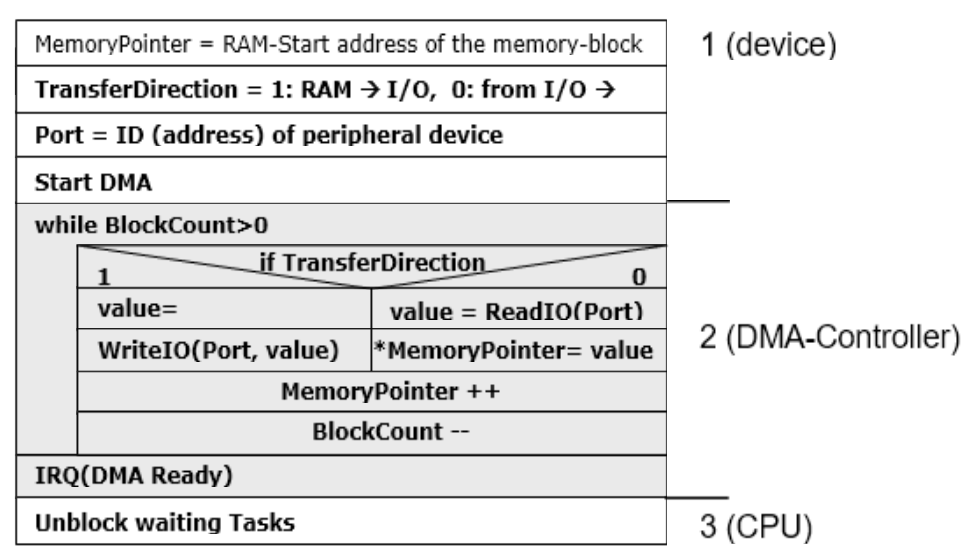
\includegraphics[width=12cm, height=6cm]{Images/image181.png}
    %\caption{}
    \label{fig:Fig 140}
    \end{figure}

Once started, the DMA controller, as a hardware component, reads data from the periphery in a loop and places them in memory (RAM), or vice versa.\\

When DMA operation three phases:

\begin{enumerate}
\item  \textbf{Initialization}: The CPU controls the bus (bus master), writes the DMA registers.
\item  \textbf{DMA operation}: The DMA controller is bus master. It transfers data between peripherals and memory. In between, the bus is given free for som time intervals. This is repeated, until all data has been transferred (this phase is often referred to as "\textbf{cycle stealing}" because the DMA controller accesses the RAM via the data bus in competition with the CPU)
\item  \textbf{End of DMA operation}: The DMA controller informs the CPU about the end by invoking an interrupt.
\end{enumerate}

DMA is used to

\begin{itemize}
\item  increase the transmission rate
\item  to relieve the CPU from trivial copy load
\end{itemize}

\textbf{Applications}: Fast peripherals, Video ADC / DAC, Audio Codecs, Hi-Speed Networks,          mass storage.

\section{Serial IO (Synchronous SPI)}

The Serial Peripheral Interface (SPI) allows synchronous communication between a master device, which provides the clock (clock), and a slave device:

    \begin{figure}[h]
    \centering
    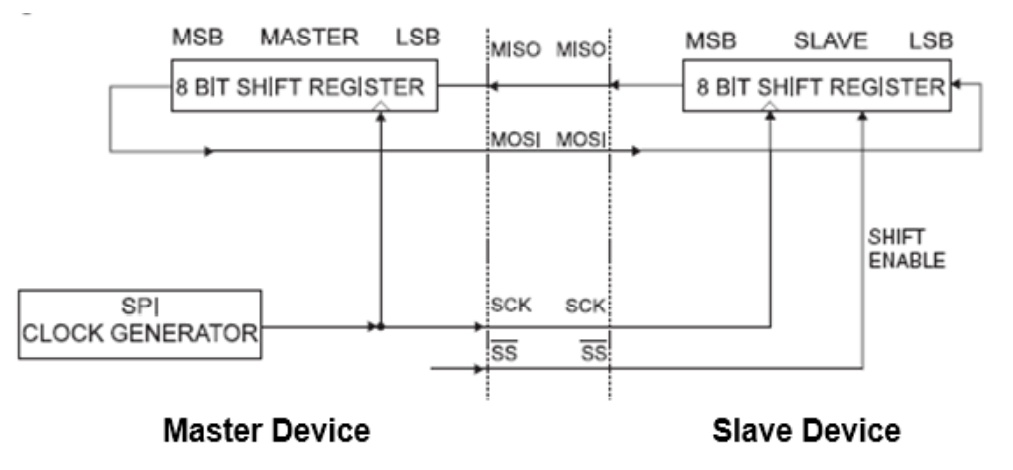
\includegraphics[width=12cm, height=5cm]{Images/image44.png}
    %\caption{}
    \label{fig:Fig 141}
    \end{figure}
    
The clock frequency can be several MHz. A microcontroller can be configured as SPI master or slave device. The physical interface consists of three or four wires / pins:\\

4 interface pins:

\begin{multicols}{2}
	\begin{itemize}
		\item  MOSI  master out slave in
		\item  MIOS  master in slave out 
	\end{itemize}
	\columnbreak
	\begin{itemize}
		\item  SCK   serial clock
		\item  SS\_n  slave select
	\end{itemize}
	\columnbreak
\end{multicols}	

3 registers are needed:

\begin{multicols}{2}
	\begin{itemize}
	\item  SPCR  control register
	\item  SPSR  status register
	\end{itemize}
	\vfill\null
	\columnbreak
	\begin{itemize}
		\item  SPDR  data register
	\end{itemize}
\end{multicols}
\textbf{Code example:}

\begin{lstlisting}[style=mystyle, language=c]
// spi_init: initializes the SPI port on the AT mega128. 
void spi_init(void){
  DDRB = DDRB | 0x07;            // Turn on SS, MOSI, SCLK (SS is output)
  SPCR |= (1<<SPEN) | (1<<MSTR); // spi enabled, master, low polarity, msb 1st
  SPSR |= (1<<SPI2X);            // run at i/o clock (fosc/128 ... fosc/2) div 2
}//spi_init

// spi_send for AT mega128 
void spi_send(uint8_t data[], uint8_t n){
  for (int i=0; i < n; i++) {
    SPDR = data[i];                     // send data byte
    while (bit_is_clear(SPSR,SPIF)) {}  // wait till data is sent out
  }
} //spi_send
\end{lstlisting}

\textbf{Example}: LTC1453 - Dual 12-Bit SAR-DAC with SPI-Interface.

\section{Serial IO (USART)}

The Universal Synchronous / Asynchronous Receiver Transmitter (UART) interface provides both, synchronous data exchange (with clock, similar to the SPI) and asynchronous data exchange without clock. The interface is used primarily as a UART (asynchronous), to implement a RS-232 or RS-485 interface

    \begin{figure}[h]
    \centering
    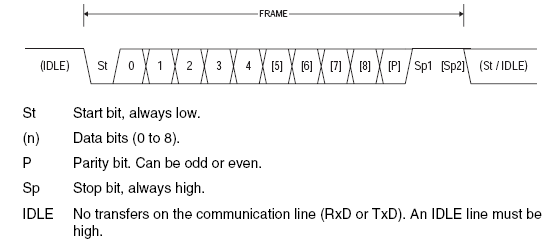
\includegraphics[width=13cm, height=5cm]{Images/image45.png}
    %\caption{}
    \label{fig:Fig 142}
    \end{figure}
 
\textbf{Typical Application of an RS-232 Interface ($\pm$ 10V) $\mu$C $\iff$ PC Communication}

    \begin{figure}[h]
    \centering
    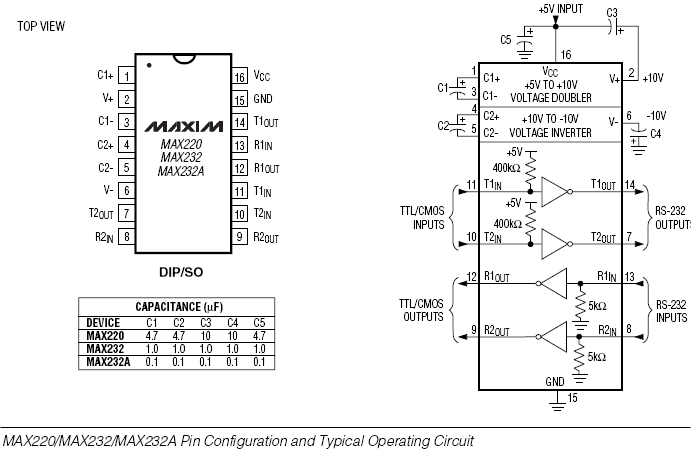
\includegraphics[width=14cm, height=12cm]{Images/image46.png}
    %\caption{}
    \label{fig:Fig 143}
    \end{figure}

For synchronization, byte by byte (or by 7-,6- or 5 bit wide words), always the beginning of the start bit is used. The baud rates can be set by the AT Mega UBRR register:

    \begin{figure}[h]
    \centering
    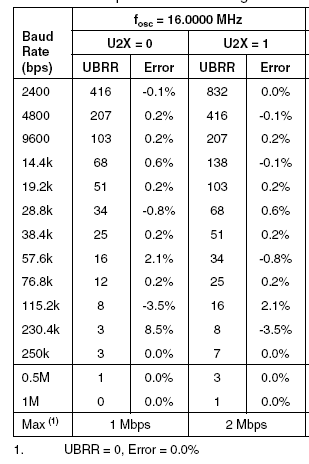
\includegraphics[width=7cm, height=7cm]{Images/image47.png}
    %\caption{}
    \label{fig:Fig 144}
    \end{figure}
\newpage
\textbf{Code Examples:}
\begin{lstlisting}[style=mystyle, language=c]
void uart_init(){
  //rx and tx enable, 8 bit characters
  UCSR0B |= (1<<RXEN0) | (1<<TXEN0);
  //async operation, no parity,  one stop bit, 8-bit characters
  UCSR0C |= (1<<UCSZ01) | (1<<UCSZ00);
  // UBRR0H=0x00; //set to 9600 baud
  // UBRR0L=0x67;
  UBRR0H=0x00; //set to 115200 baud
  UBRR0L=0x08;
  UCSRA |= (1 << U2X); // double speed mode
}

// Takes a character and sends it to USART0
void uart_putc(char data){
  while (!(UCSR0A & (1<<UDRE))); // Wait for previous transmission
  UDR0 = data;  // Send data byte
  while (!(UCSR0A & (1<<UDRE))); // Wait for previous transmission
}
// ..Modified to not block indefinately in the case of a lost byte
char uart_getc(void) {
  uint16_t timer = 0;
  while (!(UCSR0A & (1<<RXC0))) {
    timer++;
    if(timer >= 16000) return 0; // ..not block indefinately
  }  // Wait for byte to arrive
  return UDR0;
}
\end{lstlisting}

Higher Baudrates than 115.2 kBd are possible with most microcontrollers (see table above, up to 2 MBd) possible, if the physical layer is capable of higher baudrates. \\

This is true for the RS-485 interface, where the UART is used in connection with a highspeed-transceiver for tristed-pair lines for up to12 MBd:
\newpage
{\rot\bf Half-Duplex RS-485 Network with MAX488-MAX491}\\

    \begin{figure}[h]
    \centering
    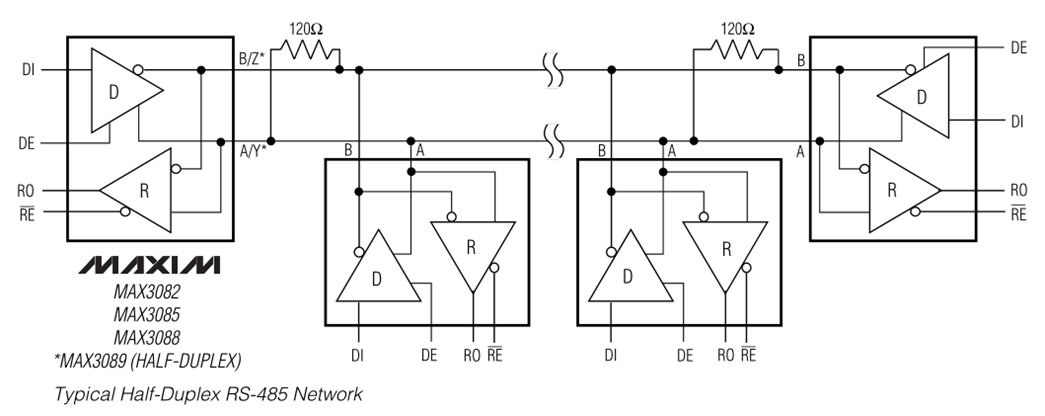
\includegraphics[width=15cm, height=6cm]{Images/image48.png}
    %\caption{}
    \label{fig:Fig 145}
    \end{figure}
    
For short line lengths USB transceivers for TTL levels (0 .. 3.3V oder 5V) are available (z.B. FT232), which can be operated at baudrates up to 2 MBd.

    \begin{figure}[h]
    \centering
    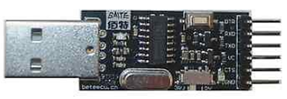
\includegraphics[width=8cm, height=2.5cm]{Images/image49.png}
    %\caption{}
    \label{fig:Fig 146}
    \end{figure}

Bluetooth-modules offer a "virtual serial interface" with baudraten up to 2~MBd either:

    \begin{figure}[h]
    \centering
    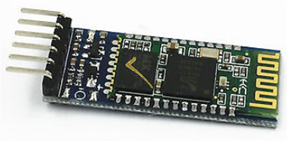
\includegraphics[width=8cm, height=2.5cm]{Images/image50.png}
    %\caption{}
    \label{fig:Fig 147}
    \end{figure}

All these UART variants can be controlled via the "Streaming API" of Unix, Windows, .. \\

\begin{lstlisting}[style=mystyle, language=c]
// open some com port ... 
hCom = CreateFile("com9", GENERIC_READ | GENERIC_WRITE, 0, NULL, ... );
...
ReadFile(hCom, buffer, sizeof(buffer), &read, NULL);     // read from com port
...
WriteFile(hCom, buffer, sizeof(buffer), &written, NULL);  // write to com port
...
CloseHandle(hCom);
\end{lstlisting}
\newpage
\section{Parallel IO (Ports)}

A pin of a microcontroller is the only \textbf{path to the process}. As only a limited number of pins is  available, the pins are designed to be as universal as possible, so that a pin can be used for various applications, such, it can be used either as input or output.\\

As the \textbf{technology of the microcontroller (CMOS)} is sensitive to electrostatic discharge (ESD) and the associated currents, there is always a \textbf{protective circuit} (diode) connected directly to the port pins:

    \begin{figure}[h]
    \centering
    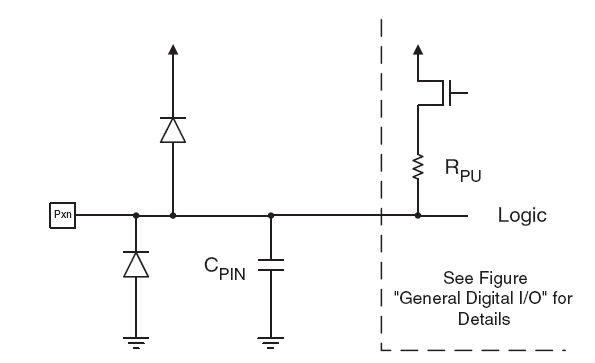
\includegraphics[width=10cm, height=6cm]{Images/image51.png}
    %\caption{}
    \label{fig:Fig 148}
    \end{figure}

It is important to note that

\begin{enumerate}
\item  the protection diodes are conductive for over voltage (Vcc + 0.6V) or low voltage (-0.6 V) and they are limited with their maximum current rating.
\item  the risk of damage by ESD at a high-impedance input port is greatest.
\item  inputs with a selectable pull-up resistor can be provided.
\item  IO ports can be usually programmed for both directions. After a reset all pins are inputs \textbf{by default}, and thus are \textbf{high impedance} (3-state) Later, at software initialization the port can be set as output (by setting bits in the Data Direction Register (DDR),  or, a pull-up resistor can be switched active.
\end{enumerate}
\newpage
{\rot\bf AVR Port Architecture:}

    \begin{figure}[h]
    \centering
    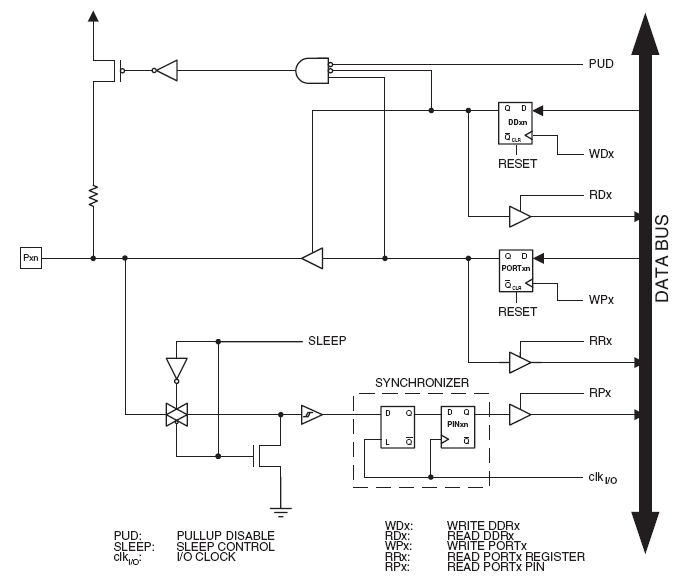
\includegraphics[width=15cm, height=12cm]{Images/image52.png}
    %\caption{}
    \label{fig:Fig 149}
    \end{figure}

All ports have

\begin{itemize}
\item  Bit selectable pull-up resistors
\item  Bit-selectable tri-state outputs
\item  Schmitt trigger input buffer
\item  Symmetrical DC Drivers
\item  Are synchronized with the internal clock
\end{itemize}